\section{useLocation}
In diesem Hook wird die aktuelle GPS-Position vom Gerät abgefragt. Der Benutzer wird, sofern er dies
noch nicht getan hat, nach der Erlaubnis gefragt, die genaue Position des Gerätes zu ermitteln und
mit der App zu teilen. Dies wird benötigt, um die Distanz zwischen Benutzer und Skateparks zu
berechnen.

In Zeile 3 wird mit Hilfe der \textbf{PermissionsAndroid}-API, bereitgestellt von React Native, überprüft,
ob die Erlaubnis schon erteilt wurde, die Position zu ermitteln.

\begin{code}[htp]
\begin{lstlisting}[firstnumber=1,language=JavaScript, style=JSX]
const checkPermission = async () => {
  if (Platform.OS === 'android') {
    const status = await PermissionsAndroid.check(
      PermissionsAndroid.PERMISSIONS.ACCESS_FINE_LOCATION,
    );

    if (status) {
      setLocError(null);
      return true;
    }
  }
  return false;
};
\end{lstlisting}
\caption{JavaScript Funktion - Berechtigung prüfen.}
\end{code}

Sollte dies nicht der Fall sein, so wird die Erlaubnis angefragt.

\begin{code}[htp]
\begin{lstlisting}[firstnumber=1,language=JavaScript, style=JSX]
const requestPermission = async () => {
  if (Platform.OS === 'android') {
    const response = await PermissionsAndroid.request(
      PermissionsAndroid.PERMISSIONS.ACCESS_FINE_LOCATION,
    );
    if (response === PermissionsAndroid.RESULTS.GRANTED) {
      setLocError(null);
      return true;
    }
  }
  setLocError('Standortdienst wurde abgelehnt');
  return false;
};
\end{lstlisting}
\caption{JavaScript Funktion - Berechtigung anfragen.}
\end{code}


\begin{figure}[H]
  \begin{center}
    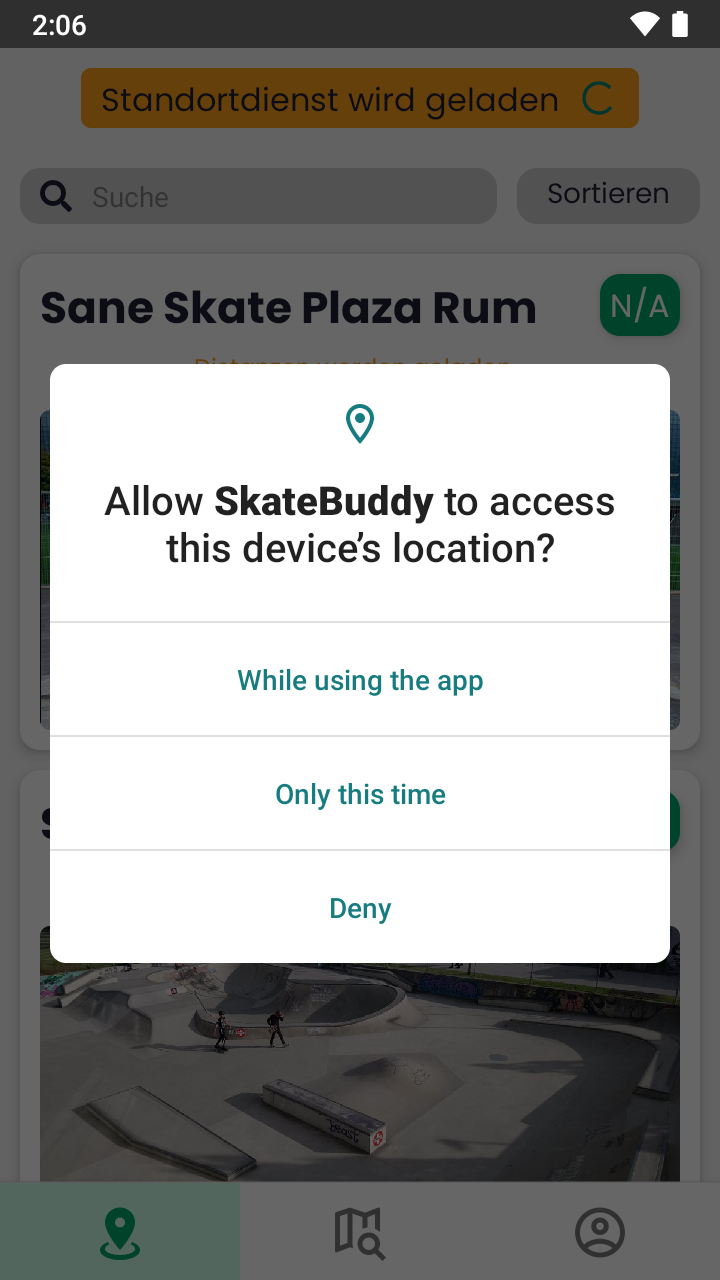
\includegraphics[width=0.6\textwidth]{Mobile/useLocationRequest.png}
    \caption{Die Berechtigungs-Anfrage beim Starten der App}
  \end{center}
\end{figure}

\begin{figure}[H]
  \begin{center}
    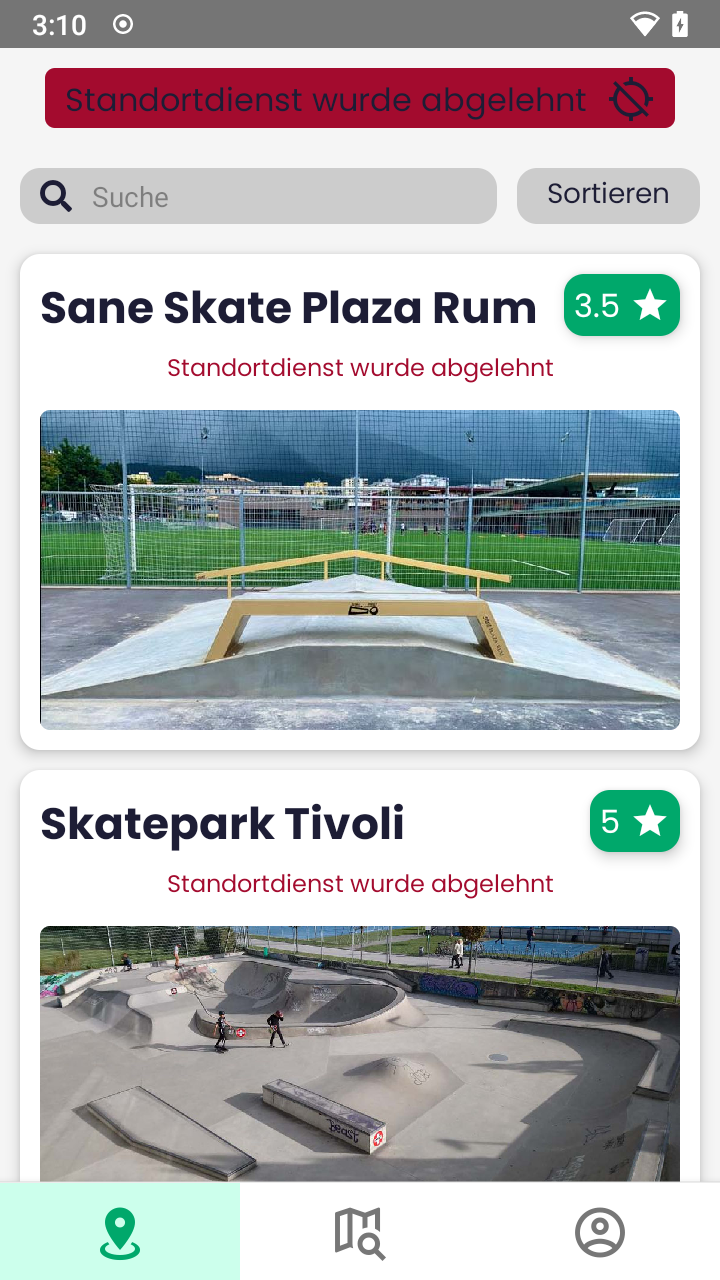
\includegraphics[width=0.6\textwidth]{Mobile/useLocationDenied.png}
    \caption{Beim Ablehnen der Aufforderung wird die Anfrage an die Directions-API abgebrochen}
  \end{center}
\end{figure}

Wenn der Benutzer den roten Knopf drückt, wird er noch einmal gebeten die Berechtigung zu erteilen.

\newpage

\begin{code}[htp]
\begin{lstlisting}[firstnumber=1,language=JavaScript, style=JSX]
const getLocation = async () => {
  setLocLoading(true);
  setLocError(null);
  if ((await checkPermission()) || (await requestPermission())) {
    Geolocation.getCurrentPosition(
      geolocation => {
        setLocation(geolocation);
        setLocLoading(false);
      },
      error => {
        setLocError(`${error.code} ${error.message}`);
        setLocLoading(false);
      },
      { enableHighAccuracy: true, timeout: 15000, maximumAge: 10000 },
    );
  }
};
\end{lstlisting}
\caption{JavaScript Funktion - Geolocation-API liefert die Position.}
\end{code}

Diese Funktion wird jedes Mal aufgerufen, um die Position zu bestimmen oder noch einmal die
Berechtigung anzufragen. Zeile 4 zeigt, dass zuerst geprüft wird, ob die Erlaubnis schon erteilt
wurde. Falls nicht wird sie angefragt. Falls dies funktioniert haben sollte, wird in Zeile 5 die
Position ausgelesen und in Zeile 7 abgespeichert. \textbf{Geolocation} ist in der Bibliothek
\textbf{react-native-geolocation-service} vorhanden.